\documentclass[11pt,a4paper]{article}
\ifdefined\pdfminorversion\pdfminorversion=7\fi
\usepackage[T1]{fontenc}
\usepackage[utf8]{inputenc}
\usepackage{lmodern}
\usepackage[a4paper,margin=25mm,headheight=14pt]{geometry}
\usepackage{amsmath,amssymb}
\usepackage{booktabs}
\usepackage{enumitem}
\usepackage{microtype}
\usepackage{tabularx}
\usepackage{xcolor}
\usepackage{pid-rs-report-tables}
\usepackage{float}
\usepackage[unicode]{hyperref}
\usepackage{xurl}
\usepackage{fancyhdr}
\usepackage{graphicx}
\usepackage{listings}
\usepackage{needspace}

\newcolumntype{L}[1]{>{\raggedright\arraybackslash}p{#1}}
\newcolumntype{Y}{>{\raggedright\arraybackslash}X}
\setlength{\emergencystretch}{3em}

\ifdefined\pdfinfoomitdate\pdfinfoomitdate=1\fi
\ifdefined\pdftrailerid\pdftrailerid{}\fi
\ifdefined\pdfsuppressptexinfo\pdfsuppressptexinfo=15\fi
\hypersetup{%
  colorlinks=true,
  pdftitle={KSG revision-4 M1a composite-v4 evidence process},
  pdfauthor={Sepehr Mahmoudian},
  pdfsubject={Append-only software-evidence contract migration},
  pdfkeywords={KSG, evidence custody, reproducibility, PID boundaries}
}

\newcommand{\Artifact}[1]{\texttt{#1}}
\newcommand{\Status}[1]{\textsf{#1}}
\newcommand{\Contract}[1]{\ensuremath{\mathsf{#1}}}
\newcommand{\Important}[1]{\textcolor{PidPrimary}{\textbf{#1}}}

\PidConfigureSections
\PidSetRunningHeads{pid-rs composite-v4}{KSG M1a evidence process}
\PidConfigureAbstract
\PidConfigureLinksAndListings

\setlength{\parindent}{0pt}
\setlength{\parskip}{5pt}
\setlist{nosep,leftmargin=5mm}
\renewcommand{\arraystretch}{1.17}

\title{\PidReportTitle
  {KSG Revision-4 M1a Composite-v4 Evidence Process}
  {An append-only repair for an uninstantiable hosted-evidence contract}}
\author{pid-rs project analysis}
\date{15 August 2026}

\begin{document}
\PidMakeTitle

\begin{abstract}
This report specifies the bounded, append-only migration from an internally inconsistent
composite-v3 hosted-evidence contract to composite-v4.  It records two separately sufficient
counterexamples, defines an acyclic two-commit topology, retains raw hosted response and artifact
bytes before deriving a typed receipt, and separates byte custody from every mathematical,
estimator, application, and scientific-novelty claim.  The frozen v3 authorities remain historical
facts; they are neither rewritten nor presented as having issued a receipt.
\end{abstract}

\begin{center}
\fcolorbox{PidAccent}{PidSoft}{\parbox{0.92\linewidth}{%
\Important{Disposition.} This document specifies project-defined process evidence. It is not a
PID definition, a KSG proof, estimator validation, peer review, authentication, attestation, or
application evidence. The frozen composite-v3 files remain historical authorities; no v3 receipt
is issued or retroactively repaired.
}}
\end{center}

\section{Why a new contract is necessary}

The recovery subject is Git commit
\path{bc3aa80fb6025e709c2906a08bce25a4fac40578}, tree
\path{7d87f87953a42edb91e40880d918471c7cbe4414}. Its hosted CI and CodeQL
runs succeeded. That success does not make every possible receipt contract satisfiable.
Composite-v3 has two separately sufficient contradictions for this exact subject.

\subsection{Opaque analysis identifiers cannot satisfy two orders}

V3 requires four CodeQL rows in semantic language order
\[
  (\text{actions},\ \text{javascript-typescript},\ \text{python},\ \text{rust})
\]
and also requires their provider analysis identifiers to be strictly increasing. The observed IDs
in that language order are
\[
  (1617732991,\ 1617732745,\ 1617735963,\ 1617735749).
\]
They are positive and unique but not increasing. Sorting the rows would violate the language
positions; moving or inventing identifiers would falsify the observation. Provider identifiers are
opaque keys, not scientific quantities. Composite-v4 therefore retains one semantic order and
requires uniqueness only within the analysis-ID resource type.

GitHub's code-scanning alert endpoints expose repository-level current state, not alerts
foreign-keyed to a workflow run and not a reconstruction of alert state during that run. The
recovery and C4 role labels group when those endpoint bytes were captured; they do not create a
run-to-alert relation. V4 deliberately requires the resulting current-state partition to equal the
retained 191-alert baseline as an operational admission condition. That equality is neither a
causal attribution to either run nor evidence about PID mathematics.

\subsection{Three additions require a fourth source-state change}

The frozen v3 direct-child rule permits exactly three additions: one receipt and two historical
index payloads. The repository-wide source-state manifest inventories every repository-visible
path except itself. Adding three paths changes the required self-excluding projection, so a truthful
child must also modify the manifest. A three-addition tree is stale; a four-path tree violates v3.
This contradiction does not rely on the CodeQL-order contradiction.

The machine-readable witness is
\nolinkurl{audit/evidence/ksg-rev4-m1a-composite-v3-impossibility-2026-08-15.json}.
It binds the frozen v3 checker, self-test, schema, current-source checker and manifest, and CI
workflow by Git blob ID, SHA-256, and byte count.

\section{Evidence ontology and custody boundary}

The durable subjects are Git commit, tree, and blob bytes; canonical manifests; exact HTTPS
response bodies; and downloaded artifact archives. A Git index is mutable local implementation
state. Two historical index hashes and sizes remain observations, but their exact bytes are no
longer available to this process. V4 neither reconstructs them nor substitutes a different index.

\begin{table}[ht]
\centering
\small
\begin{tabularx}{\linewidth}{@{}L{0.22\linewidth}Y L{0.27\linewidth}@{}}
\toprule
\PidTableHeaderRow
\textbf{Object} & \textbf{What is bound} & \textbf{What is not implied} \\
\midrule
Git object & Raw bytes rehashed under Git SHA-1; exact parent, tree, mode, and path & Repository origin, trust, authorship, or review \\
Source manifest & Full containing-tree projection except the manifest itself & Its own commit, authentication, or atomic snapshot \\
Hosted response & Two bounded response bodies, request/page identity, SHA-256, byte count & Provider authenticity, wall-clock completeness, response order \\
Artifact ZIP & API digest, exact archive bytes, safe member paths, member hashes & Semantic correctness of member content beyond named checks \\
Typed receipt & Deterministic projection re-derived from raw captures & Scientific validity, estimator quality, release readiness \\
\bottomrule
\end{tabularx}
\caption{V4 separates byte custody from scientific interpretation.}
\end{table}

\section{Acyclic two-commit topology}

\subsection{C4: contract migration}

\Contract{C4} is an unsigned, single-parent direct child of the recovery commit. It contains the v4 checker,
self-test, capture tool, closed schemas, dedicated workflow, path policy, impossibility witness,
this TeX source and PDF, bounded operational custody gates, schemas, documentation, the prospective
research-integrity workflow publication, and a separately scoped current-project Lean
replay/reseal. No KSG/PID theorem statement, scientific-object definition, numerical result, or
disposition changes, and composite-v4 derives no KSG/PID credit from that replay. C4 binds the
authored research-method bytes, but neither the v4
checker, hosted runs, nor Lean replay adjudicates the external-source observations or proves
protocol adoption. The self-excluding source manifest is generated last. C4 contains neither
hosted capture nor typed v4 receipt and therefore makes no prospective hosted-success claim.

\subsection{R4: observation receipt}

After exact-C4 hosted runs are terminal, \Contract{R4} is an unsigned, single-parent direct child of C4 with exactly
three source changes:

\begin{enumerate}
  \item add the canonical byte-retaining hosted capture;
  \item add the canonical typed receipt derived from that capture; and
  \item modify the self-excluding source manifest so it inventories both additions.
\end{enumerate}

The receipt hashes the capture but not itself, the regenerated manifest, R4's tree, or R4's commit.
Those identities are derived from Git. This orientation removes the checksum cycle while keeping
both evidence objects inside source-state custody.

\begin{figure}[ht]
\centering
% The caption and surrounding prose carry the complete semantic description.  The current PDF is
% untagged, so the source-level alt text is useful source metadata but not a PDF/UA claim.
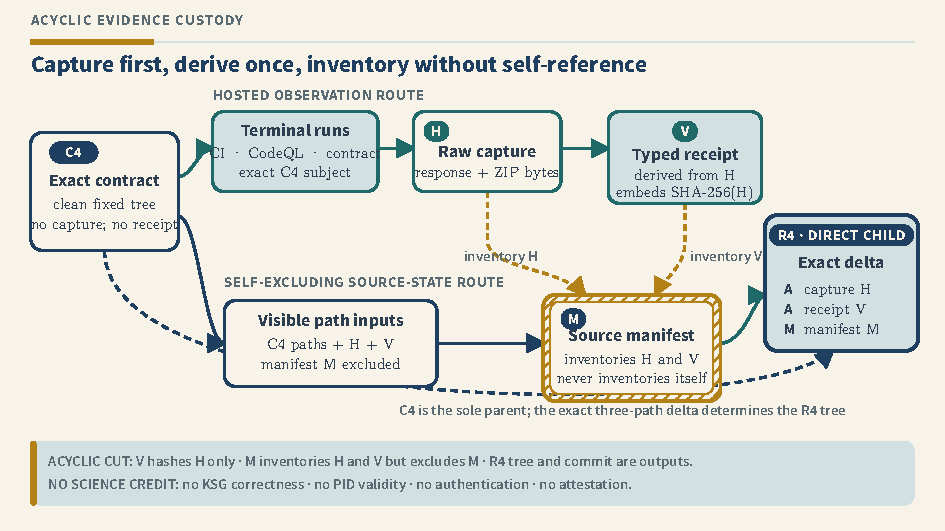
\includegraphics[
  width=\linewidth,
  alt={Acyclic C4-to-R4 custody: terminal hosted runs produce raw capture H; receipt V is derived from and hashes H; self-excluding manifest M inventories H and V; adding H, adding V, and modifying M under sole parent C4 produces R4.}
]{figures/ksg-m1a-composite-v4-process/c4-r4-acyclic-custody.pdf}
\caption{Acyclic C4-to-R4 byte custody. The typed receipt \Contract{V} is derived from the raw
capture \Contract{H} and embeds the SHA-256 digest of \Contract{H}. The self-excluding manifest
\Contract{M} inventories \Contract{H} and \Contract{V}, but never itself. \Contract{R4} is the
unsigned, single-parent direct child of \Contract{C4}; its exact tree delta adds \Contract{H}, adds
\Contract{V}, and modifies \Contract{M}. The R4 tree and commit identities are outputs, never hash
inputs. These arrows establish byte dependencies only---not KSG correctness, PID validity,
authentication, attestation, or scientific credit.}
\label{fig:c4-r4-acyclic-custody}
\end{figure}

\Needspace{14\baselineskip}
\subsection{Rejected local pre-publication replay attempt}

Before any C4 push, the first one-shot local \texttt{r9} execution and its receipt-finalization
predicates passed. The emitted canonical schema-v2 document has internal
\texttt{status = passed}; this is bounded execution-custody evidence only. The containing C4 static
check then rejected publication. For the same 748 sorted entries, the current-source generator
and first composite checker disagreed by exactly one terminal line feed:

\begin{quote}
\small\raggedright
Generator, newline-free compact JSON: 132,893 bytes.\par
SHA-256: \path{b336e6f54450090693731f2391b1ef3e112095dd9a9c8cbdadddbf2f855fba47}.\par
First composite checker, same bytes plus one terminal line feed: 132,894 bytes.\par
SHA-256: \path{7d4d4fd6bc478aeb20008cd05d1efe4b92b6ca9fd72a72043e67322e6a722f20}.
\end{quote}

Local commit \path{e02d27bec91f142949336f9f28550c672d22b297} was never pushed or accepted
as C4. The candidate receives no C4-publication, hosted, scientific, accepted-current-replay, or
independence credit. Its exact 132,710 bytes are retained unchanged:

\begin{quote}
\small\raggedright
Artifact: \path{audit/evidence/lean-4.33.0-darwin-aarch64-current-project-replay-2026-08-15-r9-prepublication-closure-rejected-2026-08-17.json}.\par
SHA-256: \path{fb162cc40da3059b61eab9024f4aa38cf6daf2d84ef7e1d8a26dc7d345291e70}.
\end{quote}

The corrected checker adopts the generator's already-published newline-free compact framing and
requires a fresh one-shot replay. The accepted \texttt{r9} slot may be filled only by a subsequent
fresh attempt over the complete corrected static-and-hostile surface, and it must bind the rejected
bytes as retained pre-publication closure evidence outside the accepted replay lineage; the
rejected document is neither renumbered nor relabelled as the current receipt. This publication
preserves the exact rejected replay and measured framing facts; it does not represent the rejected
local C4 object as a published commit.

\subsubsection{Withdrawn replay after a stale hostile fixture}

After the compact-framing repair, a fresh local replay ran from
\texttt{2026-08-17T21:20:16.677815Z} through \texttt{2026-08-17T21:36:37.989770Z} and emitted a
132,912-byte canonical schema-v2 document with internal \texttt{status = passed} and SHA-256
\path{6d5068a2ade251b4ea005e847b78be656bb7697b14ae2e6d8a644d521f09e2cb} (local Git blob
\path{3d83a833401160f8e980690b0f5d11cef5dfca19}). It bound composite checker SHA-256
\path{8640bbe11fa37011921291c719fd50bb02ac1baaf945219a4e723f46ddc7d106}. The reported local Lean
execution, receipt finalization, 114-mutation suite, and composite static checker in normal and
optimized modes passed. Before any push, the complete composite self-test stopped publication:
its \path{3f965f442fa925cd17aa466f5fee3b24207c3d2eaf98b74801c2102d48563642} fixture incorrectly
classified identical ZIP bytes delivered once directly and once through an individually safe
redirect as inconsistent. The schema and capture tool permit either delivery per request; the raw
capture hash retains the route, while repetition equality compares normalized provider semantics.

The corrected self-test, SHA-256
\path{4a40f43396e5b45aa0a5762995eabb908b61d850b1a215aa817c731140a6078b}, uses mixed direct/safe
redirect delivery as a positive and rejects a forbidden redirect host. It also makes the
repetition and duplicate-response mutations reach their named predicates rather than an earlier
workflow-name or malformed-ZIP check. Host-local commit
\path{f6d76c1d01a040f74ea55277a5ba835b32fdb6ab} with tree
\path{f5c306ab982d84d84fa47a9b4f38407bc0f843a4} and parent
\path{bc3aa80fb6025e709c2906a08bce25a4fac40578} was never pushed or accepted as C4; those local
object identities are neither a durable locator nor authentication. The candidate was not
promoted or selected and receives no C4-publication, hosted, scientific, accepted-current-replay,
selection, or independence credit. Reuse or relabelling is forbidden.

\Needspace{5\baselineskip}
C4 retains this exact identity, disposition, and omission record, but deliberately omits the
second raw preimage; its
digest alone provides neither recovery nor reproducibility. Unlike the first retained rejected
document, whose byte framing is the decisive closure witness, this second document neither caused
nor diagnosed the failure; the stale fixture and corrected causal negative are the decisive
artifacts. Reopening requires frozen corrected bytes, complete normal/optimized static and hostile
suite success, a fresh one-shot replay, current-source regeneration last, and a newly validated
exact C4.

\section{Bounded hosted-capture protocol}

Every load-bearing logical response is fetched twice. Each retained row contains the exact initial
API path, page, repetition, response kind, response SHA-256, byte count, canonical base64 body, and
redirect observation. Pagination continues through one explicit empty terminal page. Duplicate
request identities, duplicate provider resource IDs, missing pages, early empty pages, and unequal
normalized repetitions fail closed.

The bounded request set covers:

\begin{itemize}
  \item recovery and C4 CI run, complete jobs/steps, artifact listings, and every artifact ZIP;
  \item recovery and C4 CodeQL run, complete jobs, exact-head analyses, and all open, dismissed,
        and fixed alert pages; and
  \item the dedicated composite-v4 workflow run, jobs/steps, and exact static-validation ZIP.
\end{itemize}

Artifact redirects are handled explicitly. The initial authenticated request may redirect only to
a reviewed HTTPS artifact-host suffix. The authorization header is stripped before the second
request; ambient proxies are disabled. The record retains the redirect status, target host, and
SHA-256 of the full target URL, never the signed target URL itself.

Retry is narrow and observable: at most two retries for HTTP 429, 502, 503, 504, or a bounded
transport failure. Authentication, authorization, semantic, JSON, pagination, duplication, and
cardinality failures are never retried. A failed attempt contributes no observation credit.

\subsection{Executable C4-to-R4 route}

Run the following only from an exact clean C4 after all three migration runs are terminal. The
caller has already opened the GitHub token read-only on descriptor 3. Exact C4, tree, and run IDs
are supplied explicitly. The temporary parent must resolve outside the repository. A nonzero
producer exit deletes its partial standard output.

\begin{verbatim}
set -eu
repo_root=$(pwd -P)
: "${C4:?set exact C4 commit}"
: "${C4_TREE:?set exact C4 tree}"
: "${MIGRATION_CI_RUN:?set exact C4 CI run}"
: "${MIGRATION_CODEQL_RUN:?set exact C4 CodeQL run}"
: "${MIGRATION_CONTRACT_RUN:?set exact dedicated-workflow run}"
temp_parent=$(cd "${TMPDIR:-/tmp}" && pwd -P)
case "$temp_parent/" in "$repo_root/"*) exit 2 ;; esac
capture_root=$(mktemp -d "$temp_parent/pid-rs-ksg-v4-capture.XXXXXX")
chmod 700 "$capture_root"; umask 077
capture_tmp="$capture_root/capture.json.tmp"
capture="$capture_root/capture.json"
if python3 -I -S -B scripts/capture-ksg-m1a-composite-v4.py \
  --contract-commit "$C4" --contract-tree "$C4_TREE" \
  --migration-ci-run "$MIGRATION_CI_RUN" \
  --migration-codeql-run "$MIGRATION_CODEQL_RUN" \
  --migration-contract-run "$MIGRATION_CONTRACT_RUN" --token-fd 3 \
  >"$capture_tmp"; then mv "$capture_tmp" "$capture"
else status=$?; rm -f -- "$capture_tmp"; exit "$status"; fi
exec 3<&-
receipt_tmp="$capture_root/receipt.json.tmp"
receipt="$capture_root/receipt.json"
if python3 -I -S -B scripts/check-ksg-m1a-composite-v4.py \
  --derive-receipt <"$capture" >"$receipt_tmp"; then
  mv "$receipt_tmp" "$receipt"
else status=$?; rm -f -- "$receipt_tmp"; exit "$status"; fi
install -m 0644 "$capture" \
  audit/evidence/.ksg-rev4-m1a-composite-hosted-capture-v4-2026-08-15.json.tmp
mv audit/evidence/.ksg-rev4-m1a-composite-hosted-capture-\
v4-2026-08-15.json.tmp \
  audit/evidence/ksg-rev4-m1a-composite-hosted-capture-v4-2026-08-15.json
install -m 0644 "$receipt" \
  audit/evidence/.ksg-rev4-m1a-composite-receipt-v4-2026-08-15.json.tmp
mv audit/evidence/.ksg-rev4-m1a-composite-receipt-v4-2026-08-15.json.tmp \
  audit/evidence/ksg-rev4-m1a-composite-receipt-v4-2026-08-15.json
source_state_tmp="$capture_root/current-source-state-v1.json.tmp"
if python3 -I -S -B scripts/check-current-source-state-v1.py --emit \
  >"$source_state_tmp"; then
  install -m 0644 "$source_state_tmp" \
    audit/evidence/.current-source-state-v1.json.tmp
else status=$?; rm -f -- "$source_state_tmp"; exit "$status"; fi
mv audit/evidence/.current-source-state-v1.json.tmp \
  audit/evidence/current-source-state-v1.json
\end{verbatim}

The result must have exactly the three declared R4 paths. After the unsigned single-parent R4 with
exact message \texttt{Record KSG M1a composite v4 receipt}, validate its committed receipt in normal
and optimized modes:

\begin{verbatim}
python3 -I -S -B scripts/check-ksg-m1a-composite-v4.py --validate-receipt \
  <audit/evidence/ksg-rev4-m1a-composite-receipt-v4-2026-08-15.json
python3 -O -I -S -B scripts/check-ksg-m1a-composite-v4.py --validate-receipt \
  <audit/evidence/ksg-rev4-m1a-composite-receipt-v4-2026-08-15.json
\end{verbatim}

The temporary directory is not evidence. Remove it only after the committed blobs and validation
receipts are separately identified. A failed or interrupted route receives no hosted-observation
credit.

\section{Validation stack}

\begin{enumerate}
  \item \Important{Strict representation:} outer capture, receipt, counterexample, policy, and
        source-state artifacts use exact canonical serialization. Retained provider JSON remains
        byte-for-byte and is parsed as strict UTF-8 with duplicate-key, floating-point, non-finite,
        nesting, and integer-width rejection; provider formatting is not claimed canonical.
  \item \Important{Closed schema:} exact root and nested key inventories, exact JSON scalar types,
        and full semantic checks beyond what portable JSON Schema can express.
  \item \Important{Raw-to-typed join:} each raw repetition is parsed separately; run, job,
        step, artifact, analysis, and alert projections must agree exactly.
  \item \Important{Provider-resource joins:} every job binds its run, attempt, head SHA, terminal
        state, and UTC interval; every analysis records only a fixed language/category and job-name
        match, not a provider-supplied analysis-to-job foreign key.
  \item \Important{Artifact join:} archive API digest, downloaded bytes, safe ZIP members, and
        post-commit source-state fields are re-derived against the committed tree.
  \item \Important{Git graph:} raw commit, tree, and blob bytes are rehashed in process separately
        from Git-reported object IDs; C4/R4
        parentage, messages, modes, and path deltas are exact. In every checked post-R4
        descendant, exact byte retention applies to the v4-authority paths explicitly enumerated
        by the checker. Other C4 paths remain historically bound by the C4 tree and r9 map; a later
        version must be recorded by a truthfully regenerated current-source manifest rather than
        being mistaken for the original bytes.
  \item \Important{Source state:} the complete deterministic manifest is rebuilt in process
        from the containing tree, including critical artifacts, PDFs, subprojections, and nonclaims.
  \item \Important{Mutation and runtime parity:} named representative load-bearing fields receive
        type-correct, inconsistent, and unauthorized-field reseals. The exact mutation inventory,
        not this category label, defines the exercised coverage. Mixed direct and individually
        safe redirected delivery of identical ZIP bytes is a positive transport variation; an
        unsafe redirect host is the causal negative. The dedicated hosted workflow requires
        byte-identical normal and optimized Python~3.11 dispositions; broader project minor-version
        coverage is a separate CI surface and is not implied by this receipt.
\end{enumerate}

These predicates cannot detect a fully coordinated fabricated capture and matching receipt that
satisfy every declared condition; that would require a separately authenticated external anchor.
The checker therefore validates retained bytes and their deterministic interpretation without
authenticating their origin.

\section{PID and method firewall}

This contract concerns custody for one KSG M1a implementation lineage. Similar terminology does not
merge scientific objects. Each downstream claim must name its definition, estimand, support,
sample role, units, implementation route, and evidence class.

Model/agent suggestions, proof candidates, model-labelled judge outputs, and generated
certificates receive no scientific credit in C4/R4. Research/scientific or claim-adjudicating
attempts opened after this policy revision must satisfy the prospective candidate/judge controls
in \texttt{AGENTS.md} through a pre-candidate object-specific task packet and an append-only
attempt ledger covering failed and unselected attempts as well as selected successes.
C4/R4 contains no such scientific packet and makes no claim that earlier proofs or certificates
complied with that protocol.

\begin{table}[H]
\centering
\small
\footnotesize
\begin{tabularx}{\linewidth}{@{}L{0.22\linewidth}L{0.26\linewidth}Y@{}}
\toprule
\PidTableHeaderRow
\textbf{Scientific object} & \textbf{Object type} & \textbf{No-transfer boundary} \\
\midrule
Categorical MGW shared exclusions & Probability-law functional; empirical rows induce a plug-in law & Not Ehrlich continuous PID, not \(I_{\min}\), not a generic ``Wibral PID'' \\
Schick-Poland construction & General paper construction & Requires its own definition-to-route mapping \\
Ehrlich continuous shared exclusions & Analytic continuous functional & Distinct from its source-disjunction kNN estimator \\
KSG & Continuous MI estimator family & MI evidence alone does not validate any PID atom construction \\
PID2/PID3 atoms & Algebraic compositions under named redundancy terms & Algebra does not choose the redundancy functional or support contract \\
Williams--Beer \(I_{\min}\) & Distinct discrete PID & Never a fallback for MGW or Ehrlich routes \\
Fitted quantized SxPID & Project composition for a quantized estimand & Quantization changes the estimand; no continuous fallback claim \\
Infomorphic objective & Objective composed from named PID atoms & Not another PID definition; requires an explicit atom-to-objective mapping \\
\bottomrule
\end{tabularx}
\caption{Green process evidence cannot cross a scientific-object boundary.}
\end{table}

\Needspace{9\baselineskip}
\section{Research-queue non-evidence}

Deferral is not scientific rejection, but this KSG custody migration does not preserve or validate
unrelated dirty-overlay payloads.  A separate read-only work-item inventory reported a PID2
revision-3 exact-binary64/oracle candidate and a categorical SxPID3 Program-A
specification/counterexample candidate.  Their bytes are not retained by C4 or R4, so reported
fixture counts and proposed obligations are not preservation evidence here.  They remain explicit
future research items until an append-only, hash-bound intake records the exact payload,
provenance, symbol mapping, open obligations, and an explicit \texttt{absent} or \texttt{unknown}
disposition for any historical pre-candidate packet, judge, attempt ledger, and selection rule.
That intake grants no retroactive compliance credit. Every new attempt requires a newly frozen
task packet, pre-bound judge/verifier, append-only attempt ledger, and separately scoped validation
with declared independence dimensions. Those bytes are absent from C4/R4. Neither candidate may
be merged into KSG evidence or used to transfer a result between PID definitions or estimators.

\section{Reproduction and publication checklist}

\begin{enumerate}
  \item Rehash the exact recovery commit/tree and every frozen v3 authority.
  \item Run checker schema, filesystem, JSON, Git, and synthetic hosted-projection mutation suites
        under normal and optimized isolated Python. Exercise capture-tool transport security through
        its separate offline controls; do not infer a network observation from a synthetic fixture.
  \item Build this PDF with shell escape disabled; reject warnings; render every page; inspect
        clipping, overlap, glyphs, links, table width, and page order.
  \item Generate the next Lean replay only after every operational byte is quiescent and the
        generator proves the unique zero projection placeholder, both identical final
        composite-checker cuts, and the normalized three-placeholder Lean digest before any replay
        command; retain prior replay receipts append-only and validate the projection/final-custody
        cuts.
  \item Generate current-source last; deterministically reconstruct its complete containing-tree
        projection and every subprojection.
  \item Inspect the exact unsigned C4 object before fast-forward push. Require exact-SHA CI,
        CodeQL, and dedicated-v4 workflow success.
  \item Require the dedicated hosted job to contain exactly one static-validation step, one
        adversarial self-test step, and one static-artifact upload step; provider-injected setup
        steps are not substitutes for these user steps.
  \item Capture each named hosted response twice. Derive, validate, and inspect R4 before its own
        unsigned fast-forward push and exact-SHA hosted monitoring.
  \item Keep KSG revision-4 \Status{integration\_no\_go} until the separate M1c scientific packet
        closes its mathematical, implementation, numerical, statistical, and application gates.
\end{enumerate}

\section{Explicit nonclaims}

No v3 receipt is issued in the checked lineage; its reserved path remains absent from C4/R4. No historical index payload is reconstructed. No response authenticates
itself. No successful workflow is a theorem, estimator validation, peer review, release, or novelty
claim. A separate model call or model-labelled judge is not independent review. Composite-v4 does
not claim that earlier proofs, certificates, or model runs followed the prospective candidate/judge
protocol. No PID result transfers across categorical, continuous, quantized, mixed-support,
two-source, three-source, pointwise, averaged, evaluator, estimator, or objective boundaries.

\enlargethispage{3\baselineskip}
\begingroup
\footnotesize
\setlength{\parskip}{0pt}
\textbf{Bound artifact directory:} \nolinkurl{audit/evidence/}.\\
\textbf{Companion source:} \nolinkurl{ksg-rev4-m1a-composite-v4-process-2026-08-15.md};
\textbf{machine counterexample:}
\nolinkurl{ksg-rev4-m1a-composite-v3-impossibility-2026-08-15.json}.
\endgroup

\end{document}
